\chapter{An\'{a}lisis y dise\~{n}o}
%\newpage
%Cómo se plantea el desarrollo del trabajo. En que partes se 
%divide la solución, justificando dicha división y explicando 
%cada una de las partes.

%En aquellos trabajos donde sea aplicable se documentará 
%usando el modelo de dominio, el diagrama de clases, los 
%módulos/paquetes del software desarrollado, etc.

\section{An\'{a}lisis}
Los datos que ha de guardar el software estar\'an en un XML. El XML se divide en:
\begin{itemize}
	\item Observaciones
	\item Propiedades
	\item Instantes
\end{itemize}

Por tanto se ha decidido guardar la lista de Observaciones, cada observaci\'on contiene la lista de Propiedades 
y cada Propiedad una lista de Instantes en los que se guardar\'an los valores.

El rango seleccionado en cada propiedad estar\'a sincronizado con el resto de propiedades cargadas. 
Ya que no tiene sentido que por ejemplo, la observaci\'on ``coche", 
que tiene como propiedades ``velocidad" \ y ``aceleraci\'on" \ tengan distintos rangos 
seleccionados, ya que si en ``velocidad" \ seleccionamos [1, 3] y en ``aceleraci\'on" \ [2, 4], 
¿Qu\'e guardamos? ¿El primero o el segundo? Por tanto, ya que todas las propiedades suceden al
mismo tiempo se sabe que est\'an relacionadas, por lo que es necesario que los rangos est\'en
sincronizados.

A la hora de guardar, tampoco podr\'an guardarse distintos rangos que se solapen con los
previamente creados para un mismo paso o situaci\'on. La razón por la que no se pueden 
solapar es que no tiene sentido definir que algo est\'a 
ocurriendo dos veces exactamente en el mismo instante de tiempo. Si se dice que ``saltar"
se produce en el intervalo [1, 3] y en el [2, 5], en los momentos 2 y 3...
¿Se est\'a saltando dos veces? ¿Es el mismo salto? ¿Se est\'a saltando sobre un salto? ¿C\'omo 
puede ser que en medio del primer salto se defina otro salto distinto? Esa es la raz\'on principal
por la que dos cosas iguales no pueden ocurrir a la vez. En cambio, si que podr\'ia suceder
que en un mismo intervalo de tiempo est\'en sucediendo dos cosas al mismo tiempo. Por ejemplo,
``saltar" \ y ``flexionar rodillas", pero se definir\'ian como pasos diferentes.

Gr\'aficamente las clases se dividen de dos maneras: Contenedores y clases ``hoja".
El programa puede verse como una estructura de \'arbol, en las que de la ventana principal,
cuelgan los contenedores de v\'ideo y gr\'aficos, y de los de gr\'aficos cuelga el 
visualizador de datos.

Los v\'ideos tienen la misma estructura. Tambi\'en disponen de un contenedor en el que se
guardan todos los v\'ideos. Esos v\'ideos, ir\'an sincronizados con los gr\'aficos, mostrando
el progreso, para que sea m\'as intuitivo seleccionar los rangos.

\section{Dise\~{n}o}
No se ha seguido un proceso de dise\~no cl\'asico, en el cual antes de empezar a programar se realiza
un dise\~no exhaustivo, en el que se modelan las clases, atributos, incluso algunos m\'etodos y
llamadas entre m\'etodos.

Se ha seguido un proceso iterativo de dise\~no. En cada sprint, se iba construyendo sobre lo anterior, y refactorizando
y mejorando lo que hab\'ia previamente. Ha sido un proceso en el que se ha sido muy cr\'itico con lo que ya estaba
hecho, en ning\'un momento se ha dejado algo porque ``funciona", siempre se ha intentado mejorar lo que ya hab\'ia.

En cada iteraci\'on se iba consolidando el trabajo previo. Y si se llegaba a una situaci\'on en la que hab\'ia que redise\~nar
partes grandes se hac\'ia sin miedo.

\subsection{Librer\'{i}as usadas}
\begin{itemize}
    \item \textbf{AvalonDock:} 
    Es una librer\'{i}a que permite crear ventanas acoplables en WPF, al m\'as puro estilo Eclipse o Visual Studio. Es de
    c\'{o}digo abierto y gratuita, pese a que tambi\'{e}n dispone de una versi\'{o}n profesional que es de pago. La usada en este proyecto
    ha sido la versi\'{o}n gratuita o \emph{community}. La versi\'{o}n usada esta licenciada bajo licencia BSD.
    \item \textbf{OxyPlot:}
    Biblioteca de c\'odigo abierto para realizar gr\'aficos. Permite visualizar gr\'aficos cont\'inuos, discretos, 
    selecci\'on de rangos. Licenciada bajo los t\'erminos de la licencia MIT.
\end{itemize}

\subsection{Patrones utilizados}

\subsubsection{MVVM}
MVVM es un patr\'{o}n de dise\~{n}o creado por Microsoft. Intenta conseguir las ventajas de Model-View-Controller y adem\'as una separaci\'{o}n total
de la vista del controlador. De esta forma los dise\~{n}adores de UI pueden centrar todos sus esfuerzos en crear la interfaz sin preocuparse 
del c\'{o}digo de la aplicaci\'{o}n, ya que se asume que la interfaz va a cambiar mucho durante el ciclo de vida de la aplicaci\'{o}n. Pero,
¿Si separamos totalmente la vista del modelo, como se comunican? En MVC el encargado de eso es el controlador, pero un detalle importante es 
que el c\'{o}digo referente a la vista debe tener llamadas a funciones en el lenguaje utilizado.

Y en este punto es donde la parte VM \footnote{View-Model} toma sentido. El View-Model es una abstracci\'{o}n de la vista, y que es el objetivo 
de los enlaces de datos. El View-Model expone los datos del modelo para que el creador de interfaces pueda enlazar los elementos de la UI
con los datos del modelo (bien utilizando orientaci\'{o}n a objetos o exponiendo los datos de la BD) sin escribir una sola l\'{i}nea de 
c\'{o}digo .NET.

\paragraph{Elementos de MVVM}

\begin{itemize}
    \item \textbf{Model:} Dentro del patr\'{o}n MVC corresponde al modelo de dominio utilizando orientaci\'{o}n a objetos, o a los datos
    representados por una BD.
    \item \textbf{View:} La interfaz de usuario con sus botones, cajas de texto etc.
    \item \textbf{View Model:} Es la \emph{Vista del Modelo}, siendo una abstracci\'{o}n que sirve de mediadora y que expone los datos
    del modelo a la vista, para que esta \'{u}ltima pueda utilizarlas mediante enlaces de datos simples que no requieren de c\'{o}digo, sino
    que se crean mediante XAML. Realmente, no s\'{o}lo expone los datos, si no que adem\'as convierte los datos del modelo, en datos de vista, listos
    para ser visualizados.
\end{itemize}

\paragraph{Cr\'{i}ticas}
Es curioso que las principales cr\'{i}ticas provengan de su creador, Josh Gossman, el cual dice que utilizar a la fuerza MVVM para operaciones simples
de UI es una exageraci\'{o}n y que si los enlaces de datos si no se gestionan correctamente puede llevar a un consumo excesivo de 
memoria de la aplicaci\'{o}n \cite{MVVM:Criticism}

\paragraph{Uso en MIPS}
El patr\'on MVVM no se ha utilizado tal y como fue concebido. Pero s\'i se ha mantenido la separaci\'on entre
las tres partes del software. Se han creado los ViewModels tal y como se recomienda en el patr\'on, pero no
se han podido utilizar los enlaces de datos, ya que para poder usarlos hay que establecer un contexto de datos
y en este caso es din\'amico. Un contexto de datos determina de d\'onde van a obtenerse los datos para
los enlaces. Un contexto de datos puede ser el propio objeto, una lista, una consulta a una base de datos...
Y en este caso, el contexto de datos al ser din\'amico los enlaces de datos no se pueden 
establecer f\'acilmente en el XAML, hay que hacerlo
program\'aticamente. Adem\'as se necesitan m\'as cosas que simplemente visualizar unos datos. Pero
pese a todo, el software se ha construido en torno a la idea del MVVM aunque no se haya podido aplicar exactamente
como se recomienda.

\subsubsection{Iterator}
Si bien el titulo alude al patr\'{o}n \emph{Iterator} .NET no dispone como Java de las interfaces \emph{Iterable} ni
\emph{Iterator}.
En cambio, dispone de las interfaces llamadas \emph{IEnumerator<T>} e \emph{IEnumerable<T>} 
que ofrecen una funcionalidad equivalente a las de Java.

Se ha decidido utilizar este patr\'{o}n por los siguientes motivos:
\begin{enumerate}
    \item \textbf{Abstracci\'{o}n:}
    Al utilizar este patr\'{o}n se pueden obtener los elementos de un contenedor, que puede ser un \emph{array}, una \emph{LinkedList<>}...
    cualquier clase que implemente la interfaz \emph{IEnumerable<T>} sin
    exponer su representaci\'{o}n interna, aumentando la seguridad y previniendo que una clase tenga acceso a cosas que no deba.
    
    \item \textbf{Facilidad de uso:}
    Siempre es preferible utilizar cosas que nos provea el \emph{framework}, ya que no es necesario perder el tiempo en banalidades como 
    recorrer una lista, y probablemente lo haremos menos eficientemente que lo actualmente programado. De todas formas, si necesitamos
    recorrerlo de una manera particular, y que sabemos hacerlo muy eficientemente, no hay problema en no seguir el patr\'{o}n, ya que no son
    normas, si no recomendaciones.
    
    \item \textbf{Prevenci\'{o}n de errores:}
    Relacionado con lo anterior. Si se pierde el tiempo a\~{n}adiendo l\'{i}neas extra la probabilidad de que se cometa un error 
    aumenta. Y aunque no haya sido probado emp\'{i}ricamente, se tiende a pensar que \emph{¿Como me voy a equivocar en 
    recorrer un array? ¡Pero si est\'{a} perfecto!}. 
    Y ello llevar\'{a} a malgastar m\'{a}s aun algo tan preciado como el tiempo. Pero al menos servir\'a para darse cuenta del error y 
    se ver\'a lo \'{u}tiles que son los patrones.
\end{enumerate}

\paragraph{Uso en MIPS}
Este patr\'on ha sido muy \'util en todo aquello que tenga que ver con recorrer datos. Por ejemplo a la hora de
sincronizar el rango seleccionado entre los visualizadores de datos. Adem\'as en C\# se realiza de una manera 
muy sem\'antica.

\begin{lstlisting}[language=C, numbers=left, showspaces=false, breaklines=true, tabsize=2]
	public partial class UC_ChartContainer : UserControl 
	{
		private SortedSet<UC_DataVisualizer> datavisualizers;
		
		internal void updateSelections(double[] selectedRange)
		{
			foreach(UC_DataVisualizer datav in datavisualizers) 
			{
				datav.updateRangeSelection(selectedRange);
			}
		}
	}
\end{lstlisting}

Como se puede ver en el trozo de c\'odigo, se ha podido iterar a trav\'es de todos los elementos
de \emph{datavisualizers} sin tener que comprobar si hay un elemento siguiente, el tama\~no del
elemento sobre el que se quiere iterar... Y adem\'as como se ha dicho antes, este
c\'odigo se ha vuelto mucho mas legible, ya que puede leerse de la 
siguiente manera: ``para cada datav en datavisualizers,
actualizar el rango seleccionado de datav con el rango obtenido por par\'ametro".
Concretamente, el ejemplo hace referencia al m\'etodo de sincronizaci\'on de rangos de las
observaciones. Lo que se ha hecho es recorrer todas las propiedades cargadas de una observaci\'on para
sincronizarlo con el rango dado como par\'ametro.

\subsubsection{Singleton}
Patr\'on de dise\~no b\'asico que consigue que una clase tenga una \'unica instancia durante toda la ejecuci\'on del software, siendo 
accesible por toda la aplicaci\'on.

En general, hay dos maneras de crear una clase Singleton.

\paragraph{Lazy} La inicializaci\'on \emph{Lazy} o \emph{perezosa} \'unicamente crea la instancia cuando la necesita, es decir, la primera vez.
Para conseguirlo, cada vez que se intenta obtener la instancia se comprueba si ya hab\'ia sido previamente instanciada. Uno de los problemas de
la inicializaci\'on perezosa es que en entornos multihilo da problemas si no se obtiene un bloqueo exclusivo de la clase.

Una inicializaci\'on perezosa con comprobaci\'on doble de bloqueo se realiza as\'i:
\begin{lstlisting}[language=C, numbers=left, showspaces=false, breaklines=true, tabsize=2]
    public class GraphicsActions 
    {
        private static object myLock = new object();
        private static GraphicActions myGraphicActions;
        
        public static GraphicActions getMyGraphicActions()
        {
            if (myGraphicActions == null)
            {
                lock (myLock)
                {
                    if (myGraphicActions == null)
                    {
                        myGraphicActions = new GraphicActions();
                    }
                }
            }
            
            return myGraphicActions;
        }
    }
\end{lstlisting}

En .NET 4.0 fue incluida la clase \emph{Lazy<T>} que realiza ese tipo de inicializaci\'on.

\paragraph{Eager} En la inicializaci\'on \emph{Eager} o \emph{ansiosa} se crea la nueva instancia siempre. En este m\'etodo no hay problemas
en entornos multihilo, pero tiene un mayor coste computacional si la constructora es muy compleja.

Una inicializaci\'on ansiosa se realiza de la siguiente manera:
\begin{lstlisting}[language=C, numbers=left, showspaces=false, breaklines=true, tabsize=2]
    public class GraphicsActions 
    {
        private static GraphicActions myGraphicActions = new GraphicActions();
        
        public static GraphicActions getMyGraphicActions()
        { 
            return myGraphicActions;
        }
    }
\end{lstlisting}

\paragraph{Cr\'iticas}Pese a haberse utilizado el patr\'on Singleton, muchos desarrolladores desaconsejan su uso, ya que implican
una violaci\'on del Principio de Responsabilidad \'Unica del que se hablar\'a m\'as adelante. Y lo viola porque
la clase Singleton tendr\'ia dos responsabilidades, controlar que solo exista una \'unica instancia y adem\'as
toda su l\'ogica de negocio \cite{Singleton:EVIL}.

Por otro lado, tambi\'en tiene como inconveniente una de las m\'aximas de la programaci\'on: Las variables globales
son malas. Pues por si no fuera poco, un Singleton es una clase global \cite{Singleton:EVIL}.

\paragraph{Uso en MIPS}
Pese a las cr\'iticas del p\'arrafo anterior, se ha utilizado en aquellos elementos que solo iban a tener
una instancia. Concretamente \emph{VideoActions}, \emph{GraphicActions} y \emph{XMLExport}. Al
hacerlos accesibles desde todo el c\'odigo, se ha facilitado mucho la tarea al desarrollador para utilizarlo.

\subsection{SOLID}
SOLID es un acr\'{o}nimo mnem\'{o}nico acu\~{n}ado a comienzos de la d\'{e}cada de los 2000 por 
Robert C. Martin \cite{SOLID:ADefinition}
que representa cinco principios b\'{a}sicos de la programaci\'{o}n orientada a objetos y del dise\~{n}o de software.

SOLID merece un apartado en esta memoria ya que se ha intentado cumplir en el mayor grado posible los cinco principios.

Los principios son los siguientes:
\subsubsection{Single responsibility principle}
Traducido al castellano: Principio de responsabilidad \'{u}nica. El nombre puede llevar a enga\~{n}o ya que Martin define como 
\emph{responsabilidad}
a una \emph{raz\'{o}n de cambio} \cite{SOLID:SRP} y concluye que una clase, debiera tener, una, y solamente una raz\'{o}n 
para cambiar.

Por ejemplo, imaginemos que disponemos de una clase, o m\'{o}dulo que compila e imprime un informe. 
Ese informe puede cambiar por dos razones, de estilo, o de contenido. 

El principio de responsabilidad \'{u}nica dice que una clase solo debiera cambiar por un motivo, y por 
tanto tendr\'{i}amos que separar el m\'{o}dulo en dos: El que compila el informe, y el que lo imprime.

Utilizando este principio volveremos nuestro c\'{o}digo m\'as robusto, ya que un cambio en una clase, no 
deber\'{i}a afectar a la salida, y por tanto los siguientes m\'{o}dulos que se alimenten de esa clase.

\paragraph{Uso en MIPS}
Si bien el principio de responsabilidad \'unica no es algo que se aplique de manera directa, es decir,
no es si sucede A entonces haz B. Pero hay en algunas situaciones en las que se cumple este principio.
Por ejemplo, en la clase \emph{UC\_ChartContainer} se manten\'ia un repositorio de Observaciones
y adem\'as de propiedades. Se ve, que esta clase tiene dos razones de cambio. Una es por las propiedades
(a\~nadir, borrar etc) y la otra por las observaciones (a\~nadir, borrar etc). Al incumplirse el principio,
la clase ha de separarse en dos. En un repositorio de propiedades, y en un repositorio de observaciones.

En este caso concreto, no se separ\'o en dos clases, sino que la colecci\'on de propiedades, pas\'o a ser
responsabilidad de cada \emph{UC\_ChartContainer}.

\subsubsection{Open/Closed principle}
El principio abierto / cerrado \cite{SOLID:OCP} implica que una clase est\'{a} abierta a la extensi\'{o}n pero cerrada a la 
modificaci\'{o}n. Ya que un cambio en el
funcionamiento de una clase har\'{i}a que se tambalease la estabilidad de nuestro software.

\paragraph{Uso en MIPS}
Ciertamente este principio no se ha utilizado, ya que est\'a m\'as pensado para ser usado en
c\'odigo que ya est\'a en producci\'on, no mientras el software est\'a en desarrollo.

\subsubsection{Liskov's substitution principle}
El principio de sustituci\'{o}n de Liskov \cite{SOLID:LSP} \footnote{\url{http://pmg.csail.mit.edu/~liskov/}} 
sostiene que cualquier subtipo de una clase
debe poder sustituir a su supertipo sin que haya un cambio de comportamiento.

M\'{a}s formalmente: Si \textbf{S} es un subtipo de \textbf{T} entonces \textbf{T} puede sustituirse por \textbf{S} y 
conservar su exactitud, tarea que realiza etc.

\paragraph{Uso en MIPS}
Este principio se cumple claramente, ya que para incumplirlo habr\'ia que sobreescribir alg\'un m\'etodo de la superclase
y que funcionase diferente de como funciona en la superclase. 

T\'omese como ejemplo las clases \emph{XMLValidation} y \emph{XMLLoader}.
Si \emph{XMLValidation} no fuera abstracta, podr\'ia ser sustituida por \emph{XMLLoader}
sin alterar su funcionalidad base, ya que \emph{XMLLoader} no sobreescribe el m\'etodo de la clase base. Lo mismo
sucede con los ViewModels. Ambas clases derivadas podr\'ian sustituir a la clase abstracta sin cambiar su funcionalidad. Es
decir, aunque las clases derivadas hayan sustituido a la clase padre, las clases derivadas siguen teniendo la funcionalidad
de la clase base intacta.

\subsubsection{Interface segregation principle}
El principio de segregaci\'{o}n de interfaces dice que es mejor tener muchas interfaces espec\'{i}ficas, 
que una gran interfaz que contenga todo \cite{SOLID:ISP}.

De esta manera evitamos que haya partes del software que dependan de m\'{e}todos que no influyen en esa clase.

\paragraph{Uso en MIPS}
Al solo tener una interfaz propia, y que adem\'as tiene un \'unico m\'etodo, se cumple siempre, ya que
cada vez que una clase implemente esa interfaz es porque se requiere ese m\'etodo, si no, no tendr\'ia sentido
implementarla.

\subsubsection{Dependency inversion principle}
El principio de Inversi\'{o}n de dependencia \cite{SOLID:DIP} dice que:
\begin{enumerate}
    \item Los m\'{o}dulos de alto nivel no deben depender en m\'{o}dulos de bajo nivel. Ambos deben depender de abstracciones
    \item Las abstracciones no deben depender en los detalles. Los detalles deben depender de las abstracciones.
\end{enumerate}

\paragraph{Uso en MIPS}
Este principio es el \'unico que no se cumple. Ya que los m\'odulos de alto nivel, como por ejemplo
\emph{UC\_ChartContainer} no depende de abstracciones, sino de tipos concretos (\emph{UC\_DataVisualizer}).
Para arreglarlo, habr\'ia que definir una serie de interfaces que describan los m\'etodos necesarios que 
debe tener un visualizador de datos. Y de esa manera el contenedor depende de esas abstracciones (interfaces).
Esto mismo habr\'ia que aplic\'arselo a todos los elementos del proyecto.

Excepto en casos muy concretos, los m\'etodos, deber\'ian tomar como par\'ametros, o bien interfaces, o bien
objetos que implementen esas interfaces.

\subsection{Clean Code}
Otra de las cosas en las que incide mucho Martin es que evitemos realizar comentarios en el c\'odigo,
ya que el hecho de realizar un cambio en el c\'odigo no garantiza que vayamos a cambiar el comentario, y 
puede llevar a errores futuros o a inconsistencias en la documentaci\'on. Adem\'as, todo el mundo sabe que programar
es un arte \cite{Art:Programming}, y es por ello que el c\'odigo de MIPS tiene los comentarios justos y necesarios
para hacer entender los m\'etodos que no se entienden o que tienen una l\'ogica ligeramente mas compleja de seguir.

\subsection{Diagrama de clases}
El diagrama de clases \ref{fig:ClassDiagram} tiene todos los m\'etodos, propiedades y atributos ocultos para que entrase
en el propio documento. En el anexo \ref{chap:DiagramaDeClasesCompleto} puede encontrarse la versi\'on completa. Las clases que no son descritas m\'as adelante es porque o bien
son clases propias de .NET o porque son clases generadas por Visual Studio.

\begin{figure}[H]
	\centering
	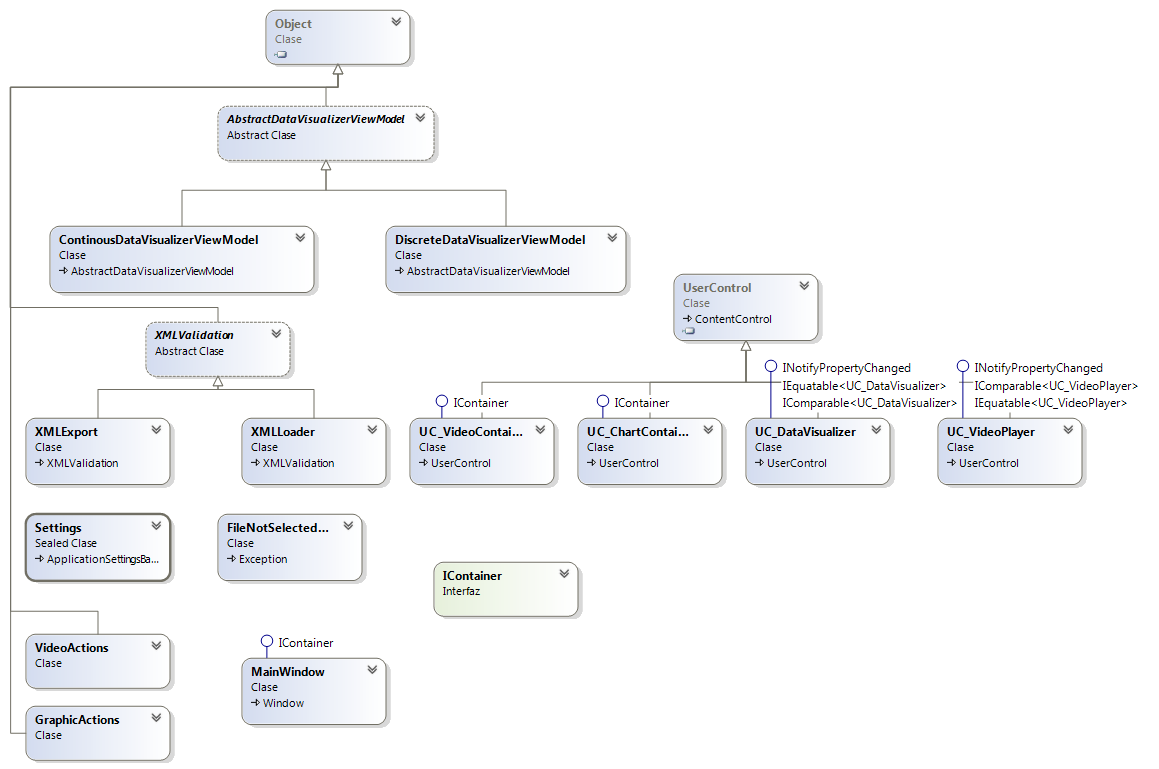
\includegraphics[width=1.2\linewidth]{./Figures/ClassDiagram}
	\caption[Diagrama de clases compacto]{Diagrama de clases compacto}
	\label{fig:ClassDiagram}
\end{figure}

\subsubsection{AbstractDataVisualizerViewModel}
Clase abstracta que describe e implementa todos los m\'etodos y propiedades que han de tener todos los ViewModels. Es decir,
define todo aquello que podr\'a ser cargado por un \emph{UC\_DataVisualizer}. Esta clase expone el m\'etodo
\emph{potected abstract PlotModel createModel(List<DataPoint> points)}
que todas sus subclases han de implementar.

\subsubsection{ContinousDataVisualizerViewModel}
Subclase de \emph{AbstractDataVisualizerViewModel} que se especializa en tratar los datos cont\'inuos. 

\subsubsection{DiscreteDataVisualizerVIewModel}
Subclase de \emph{AbstractDataVisualizerViewModel} que se especializa en tratar los datos discretos.
Esta clase requiere de datos adicionales, concretamente los elementos del eje de ordenadas.

\subsubsection{XMLValidation}
Clase abstracta que sirve como base a todas aquellas clases que requieran de validar un XML contra un XSD.

\subsubsection{XMLExport}
Subclase de \emph{XMLValidation} que se encarga de gestionar todo lo relacionado con exportar un XML. Creaci\'on y
validaci\'on de intervalos y guardar a disco el paso o situaci\'on principalmente.

\subsubsection{XMLLoader}
Subclase de \emph{XMLValidation} que tiene como responsabilidad cargar los datos del XML, tanto obtener los datos
para mostrar en el \'arbol como de crear los ViewModels que despu\'es ser\'an utilizados por los \emph{UC\_DataVisualizer}.

\subsubsection{VideoActions}
Clase Singleton que proporciona los m\'etodos necesarios para gestionar los v\'ideos cargados.

\subsubsection{GraphicActions}
Clase Singleton que gestiona los \emph{UC\_ChartContainer}. A\~nadir, borrar, sincronizar rangos etc.

\subsubsection{UC\_VideoContainer}
Control de usuario derivado de \emph{UserControl} y que implementa
la interfaz \emph{IContainer}. Dispone de la interfaz y los m\'etodos necesarios para
gestionar los \emph{UC\_VideoPlayer} (a\~nadir, borrar etc) as\'i como unos controles globales
para controlar su reproducci\'on.

\subsubsection{UC\_ChartContainer}
Control de usuario derivado de \emph{UserControl} y que implementa la interfaz
\emph{IContainer}. Esta clase contiene la interfaz gr\'afica y los m\'etodos requeridos para gestionar
los \emph{UC\_DataVisualizer}. Representa una observaci\'on que dentro tiene sus propiedades.
Tambi\'en es importante a\~nadir que es esta clase la que se suscribe al evento que notifica
que el rango seleccionado ha cambiado, para poder inicial el proceso de sincronizaci\'on.

\subsubsection{UC\_DataVisualizer}
Control de usuario que se encarga de mostrar los datos de las propiedades y una de las funcionalidades
principales consiste en notificar a su padre (un \emph{UC\_ChartContainer}) de que el rango seleccionado ha cambiado.

Esta clase extiende a \emph{UserControl} e implementa las interfaces \emph{INotifyPropertyChanged},
\emph{IEquatable<T>} e \emph{IComparable<T>}. Es necesario implementar
esas interfaces para que el \'arbol d\'onde se almacenan los objetos funcione correctamente, ya que 
requiere ordenar las instancias
de alguna manera. 

\subsubsection{UC\_VideoPlayer}
Control de usuario que se encarga de reproducir v\'ideos.

Al igual que \emph{UC\_DataVisualizer} extiende \emph{UserControl} 
e implementa las interfaces \emph{INotifyPropertyChanged},
\emph{IEquatable<T>} e \emph{IComparable<T>}. Los motivos de su implementaci\'on
son los mismos que en \emph{UC\_DataVisualizer}.

\subsubsection{IContainer}
Esta interfaz define aquellos m\'etodos que deben ser implementados por las clases que vayan a ser contenedores
de alg\'un tipo de dato.

\subsubsection{FileNotSelectedException}
Excepci\'on personalizada pensada para ser lanzada en los di\'alogos de apertura de ficheros.

\subsubsection{MainWindow}
Punto de entrada al programa. Al ser un contenedor de contenedores, concretamente de \emph{UC\_ChartContainer} y
\emph{UC\_VideoContainer}, tambi\'en implementa la interfaz \emph{IContainer}.

Esta clase, principalmente se encarga de realizar las llamadas a cargar los datos y añadir las observaciones
y el contenedor de v\'ideos.